% СПО ЛКС - Сокеты
% Пынькин Д.А. (с) 2011
\documentclass[ignorenonframetext, hyperref={pdftex, unicode}]{beamer}
\usepackage{beamerthemesplit}

\usetheme{Pittsburgh}
\usecolortheme{dolphin}

\usepackage[russian]{babel}
\usepackage[utf8]{inputenc}
\usepackage[T1]{fontenc}
\usepackage{ulem}
%\usepackage{html}

\usepackage{verbatim}

\usepackage{tikz}
\usetikzlibrary{positioning,arrows}

\title[СПОЛКС (http://goo.gl/32cTB)]{Системое программное обеспечение локальных компьютерных сетей}
\author{Денис Пынькин}
\date{2011 -- 2012}
%\institution[БГУИР]{Белорусский государственный университет информатики и радиоэлектроники}
%\logo{
\includegraphics[width=1cm]{logo-kafEVM.png}}


\subtitle{Программный интерфейс взаимодействия сокетов Беркли\\(проолжение)}

\begin{document}

\mode<all>{\begin{frame}
\titlepage
\begin{center}
e-mail: denis.pynkin@bsuir.by\\
\end{center}
\begin{center}
{\bfseries http://goo.gl/32cTB}

{\tiny СЧАСТЬЕ ДЛЯ ВСЕХ, ДАРОМ, И ПУСТЬ НИКТО НЕ УЙДЕТ ОБИЖЕННЫЙ!\\
(c)Стругацкие, Пикник на обочине}
\end{center}
\end{frame}
}

%
% Далее начинается сама презентация
%
%\section{}

\section{Базовые сетевые функции}
\begin{frame}{Сетевое взаимодействие}
	\begin{columns}
	\column{0.5\textwidth}
	\begin{center}
		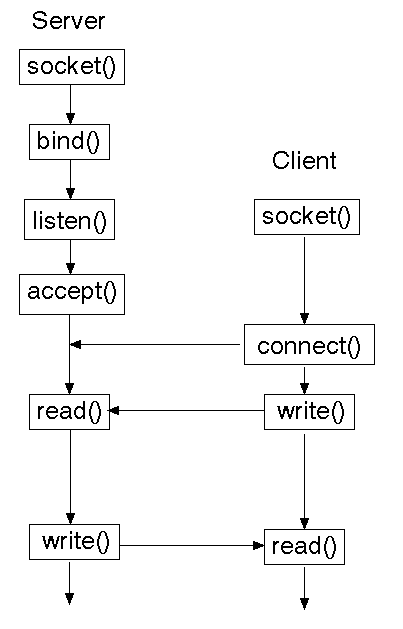
\includegraphics[height=0.8\textheight]{06-tcp_seq.png}
	\end{center}
	\column{0.5\textwidth}
	\begin{center}
		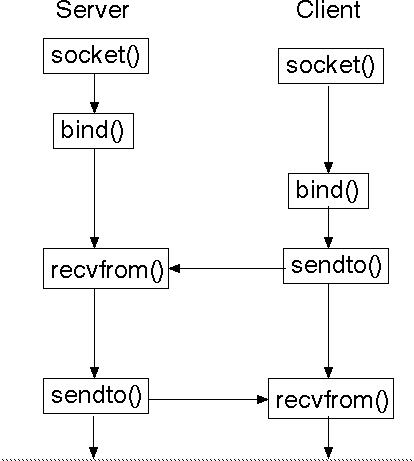
\includegraphics[height=0.6\textheight]{06-udp_seq.png}
	\end{center}

\end{columns}
\end{frame}

\begin{frame}[fragile]{socket}

{\tt socket} -- создать оконечную точку коммуникации   

\scriptsize\begin{lstlisting}[language=C]
#include <sys/types.h> 
#include <sys/socket.h> 
int socket(int domain, int type, int protocol);   
\end{lstlisting}

Вызов {\tt socket} создает оконечную точку для коммуникации и возвращает её дескриптор.\\
В случае ошибки возвращается -1; в противном случае возвращается дескриптор, ссылающийся на сокет. 
\end{frame}

\begin{frame}{Домен коммуникации}
Параметр {\tt domain} задает ``домен'' коммуникации; выбирает набор протоколов, которые будут использоваться для коммуникации.

Такие наборы описаны в <sys/socket.h>. Примеры форматов: 

\begin{itemize}
\item PF\_UNIX,PF\_LOCAL -- Локальная коммуникация
\item PF\_INET --	IPv4, протоколы Интернет
\item PF\_INET6 -- IPv6, протоколы Интернет
\item PF\_IPX -- IPX -- протоколы Novell
\item PF\_NETLINK -- Устройство для общения пользователя с ядром
\item PF\_X25 -- Протокол ITU-T X.25 / ISO-8208
\item PF\_AX25 -- Протокол AX.25, любительское радио 
\item PF\_APPLETALK -- Appletalk
\item PF\_PACKET -- Низкоуровневый пакетный интерфейс
\end{itemize}
\end{frame}

\begin{frame}{Тип сокета}
Сокет имеет тип {\tt type}, задающий семантику коммуникации. Стандарт POSIX определяет следующие типы:

\begin{itemize}
	\item SOCK\_STREAM 
	\item SOCK\_SEQPACKET
	\item SOCK\_DGRAM
	\item SOCK\_RAW
\end{itemize}
\end{frame}

\begin{frame}{Протокол сокета}
Параметр {\tt protocol} задает конкретный протокол, который используется на сокете. 
Обычно существует только один протокол, обеспечивающий конкретный тип сокета в 
заданном наборе протоколов. Однако, возможно существование нескольких таких 
протоколов -- тогда и используется этот параметр. 
Номер протокола зависит от используемого домена коммуникации.
\end{frame}

\begin{frame}[fragile]{socketpair}

{\tt socketpair} -- создать неименованную пару подключенных сокетов (аналог неименованных каналов через сокеты)

\scriptsize\begin{lstlisting}[language=C]
#include <sys/types.h> 
#include <sys/socket.h> 
int socketpair(int domain,  int type, int protocol, int sv[2]);
\end{lstlisting}

Вызов {\tt socketpair} создает неименованную пару подключенных оконечных точек для коммуникации и возвращает их дескрипторы.
\end{frame}


\begin{frame}[fragile]{bind}

{\tt bind} -- привязать имя к сокету
\scriptsize\begin{lstlisting}[language=C]
#include <sys/types.h>
#include <sys/socket.h>

int bind(int sockfd,  struct sockaddr *my_addr,  socklen_t addrlen);
\end{lstlisting}
{\tt bind} привязывает  к  сокету  {\tt sockfd} локальный адрес {\tt my\_addr} длиной {\tt addrlen}.  Традиционно, эта операция называется ``присваивание сокету имени''.
\end{frame}

\begin{frame}[fragile]{listen}

{\tt listen} -- слушать соединения на сокете (перевести сокет в пассивный режим).

\scriptsize\begin{lstlisting}[language=C]
#include <sys/socket.h> 
int listen(int s, int backlog);   
\end{lstlisting}
В случае успеха возвращается нуль. 
При ошибке возвращается -1, а {\tt errno} устанавливается должным образом.
\end{frame}

\begin{frame}{listen}

Системный вызов {\tt listen} применим 
только к сокетам типа {\tt SOCK\_STREAM} или {\tt SOCK\_SEQPACKET}.

Параметр {\tt backlog} задает максимальную длину, до которой может расти очередь 
ожидающих соединений. Если приходит запрос на соединение, а очередь полна,
то клиент получит ошибку {\tt ECONNREFUSED} или, если соответствующий
протокол поддерживает повторную передачу, запрос может быть игнорирован,
чтобы попытаться ответить на повторный запрос.   
\end{frame}

\begin{frame}[fragile]{accept}

{\tt accept} -- прием соединений
\scriptsize\begin{lstlisting}[language=C]
#include <sys/socket.h>
int accept (int sd,  struct sockaddr *restrict address, 
       socklen_t *restrict address_len);
\end{lstlisting}
Этот системный вызов возвращает -1 в случае  ошибки.   При  успешном  завершении  возвращается  неотрицательное целое,  являющееся дескриптором сокета.
\end{frame}

\begin{frame}[fragile]{connect}

{\tt connect} -- инициирует соединение на сокете.

\scriptsize\begin{lstlisting}[language=C]
#include <sys/types.h> 
#include <sys/socket.h> 
int connect(int sockfd, const struct sockaddr *serv_addr, socklen_t addrlen); 
\end{lstlisting}

Если соединение или привязка прошла успешно, возвращается нуль. 
При ошибке возвращается -1, а {\tt errno} устанавливается должным образом.
\end{frame}

\begin{frame}{connect}
Файловый дескриптор {\tt sockfd} должен ссылаться на сокет. 
Если сокет имеет тип {\tt SOCK\_DGRAM}, значит, адрес {\tt serv\_addr} является 
адресом по умолчанию, куда посылаются датаграммы, и единственным адресом, откуда 
они принимаются. Если сокет имеет тип {\tt SOCK\_STREAM} или {\tt SOCK\_SEQPACKET},
то данный системный вызов попытается установить соединение с другим сокетом.
Другой сокет задан параметром {\tt serv\_addr}, являющийся адресом длиной 
{\tt addrelen} в пространстве коммуникации сокета. Каждое пространство коммуникации 
интерпретирует параметр {\tt serv\_addr} по-своему.
\end{frame}

\begin{frame}{connect}
Обычно сокеты с протоколами, основанными на соединении, могут устанавливать 
соединение только один раз; сокеты с протоколами без соединения могут 
использовать {\tt connect} многократно, чтобы изменить адрес назначения. 
Сокеты без поддержки соединения могут прекратить связь с другим сокетом, 
установив член {\tt sa\_family} структуры sockaddr в {\tt AF\_UNSPEC}.
\end{frame}


\begin{frame}[fragile]{send}

{\tt send, sento, sendmsg} -- отправить сообщение в сокет 
\scriptsize\begin{lstlisting}[language=C]
#include <sys/types.h>
#include <sys/socket.h>

int send(int s,  const void *msg,  size_t len,  int flags);
int sendto(int s,  const void *msg,  size_t len,  int flags,
		const struct sockaddr *to,  socklen_t tolen);
\end{lstlisting}
{\tt send}, {\tt sendto},  и {\tt sendmsg} используются для пересылки сообщений  на  другой  сокет. {\tt send}  можно использовать,   только если сокет находится в соединенном состоянии,  тогда как {\tt sendto} и {\tt sendmsg} можно использовать в любое время.

Эти системные вызовы возвращают  количество  отправленных  символов  или  -1, если  произошла ошибка.
\end{frame}

\begin{frame}[fragile]{recv}

{\tt recv,  recvfrom,  recvmsg} -- получить сообщение из сокета
\begin{lstlisting}[language=C]
#include <sys/types.h>
#include <sys/socket.h>

int recv(int s, void *buf, size_t len, int flags);
int recvfrom(int s, void *buf, size_t len, int flags,
		struct sockaddr *from, socklen_t *fromlen);
\end{lstlisting}
Системные вызовы {\tt recvfrom} и {\tt recvmsg} используются для получения сообщений из  сокета, и  могут
использоваться  для получения данных,  независимо от того,  является ли сокет ориентированным на
соединения или нет.
\end{frame}

\begin{frame}{Флаги}
	\begin{itemize}
	\item MSG\_OOB -- Запрашиваются экстренные данные. Трактовка этого понятия зависит от протокола.
	\item MSG\_DONTROUTE (send) -- не использовать  маршрутизацию  при  отправке пакета
	\item MSG\_DONTWAIT (send) -- включает неблокирующий режим
	\item MSG\_TRUNC (recv) -- Возвращает реальную длину пакета (пакетные протоколы) 
	\item MSG\_PEEK (recv) -- Не удалять прочитанные данные.
	\item MSG\_WAITALL (recv) -- для сокетов типа SOCK\_STREAM флаг означает,  что вызывающий процесс блокируется до получения всего запрошенного объема данных.
	\end{itemize}
\end{frame}

\begin{frame}[fragile]{close}

{\tt close} -- закрыть файловый дескриптор
\begin{lstlisting}[language=C]
#include <unistd.h>

int close(int fd);
\end{lstlisting}
возвращает ноль при успешном завершении или -1,  если произошла ошибка.
\end{frame}

\begin{frame}[fragile]{shutdown}

{\tt shutdown} -- закрыть файловый дескриптор
\begin{lstlisting}[language=C]
#
#include <sys/socket.h>
int shutdown (int sd,  int how);
\end{lstlisting}
возвращает ноль при успешном завершении или -1,  если произошла ошибка.

Значение аргумента how показывает,  что именно завершается: {\tt SHUT\_RD} прекращает прием, {\tt SHUT\_WR} -- отправку, {\tt SHUT\_RDWR} -- и то, и другое.
\end{frame}

\begin{frame}[fragile]{select}

Функции {\tt select} и {\tt pselect} ждут изменения статуса нескольких файловых дескрипторов
\begin{lstlisting}[language=C]
#include <sys/time.h>
#include <sys/types.h>
#include <unistd.h>

int select(int n,  fd_set *readfds,  fd_set *writefds,  
  fd_set *exceptfds,  struct timeval  *timeout);
\end{lstlisting}
\end{frame}

\begin{frame}[fragile]{select}

	{\tt n} на единицу больше самого большого номера дескриптора из всех наборов.
	\bigskip
	{\tt timeout} --  это  верхняя  граница  времени,  которое пройдет перед возвратом из select.  
	Можно использовать ноль,  при этом select завершится немедленно.   (Это  полезно  для  периодического
	опроса.)   Если  timeout  равен  NULL  (нет  тайм-аута),   то  select  будет  
	ожидать изменений неопределенное время.

\end{frame}

\begin{frame}[fragile]{fd\_set}

Стандарт POSIX-2001 определяет тип {\tt fd\_set} как абстрактный.

\begin{lstlisting}[language=C]
FD_SET(int fd,  fd_set *set);
FD_CLR(int fd,  fd_set *set);
FD_ISSET(int fd,  fd_set *set);
FD_ZERO(fd_set *set);
\end{lstlisting}

\end{frame}


\begin{frame}[fragile]{Опции сокетов}
С сокетами могут быть ассоциированы опции,  влияющие на их функционирование. Значения этих опций можно опросить или изменить с помощью функций {\tt getsockopt} и {\tt setsockopt}.
\begin{lstlisting}[language=C]
#include <sys/socket.h>
int getsockopt (int sd,  int level,  
  int option_name,  
  void *restrict option_value,  
  socklen_t *restrict option_len);

int setsockopt (int sd,  int level,  
  int option_name,  
  const void *option_value,  
  socklen_t option_len);
\end{lstlisting}

\end{frame}

\begin{frame}{Уровни опций}

	{\tt level} -- указывает к какому уровню относится опция

	\begin{itemize}
		\item SOL\_SOCKET -- опции сокета
		\item SOL\_TCP -- опции для протокола TCP
		\item SOL\_IP -- опции для протокола IP
	\end{itemize}
\end{frame}

\begin{frame}{SOL\_SOCKET}

\scriptsize
	\begin{table}[ht]
	\centering
	\begin{tabular}[c]{l|c|l}
Имя опции & Тип & Описание \\
	\hline
SO\_ERROR & int & Статус ошибок (после опроса очищается)\\
SO\_TYPE & int & Тип сокета\\
SO\_PROTOCOL & int & Протокол \\
SO\_DEBUG & bool & Отладочная информация о работе сокета.\\
SO\_ACCEPTCONN & bool & Указывает,  является ли сокет слушающим. \\
SO\_SNDBUF & int & Размер буфера для передаваемых данных (выходного буфера)\\
SO\_RCVBUF & int & Размер входного буфера. \\
SO\_RCVLOWATM & int & Минимальное число байт,  обрабатываемых при вводе.\\
SO\_SNDLOWAT & int & Минимальное число байт,  обрабатываемых при выводе. \\
SO\_RCVTIMEO & timeval & Длительность ожидания поступления данных при вводе.\\
SO\_SNDTIMEO & timeval & Длительность ожидания отправки данных при выводе. \\
SO\_TIMESTAMP & bool & Включить передачу отметок времени \\
SO\_BROADCAST & bool & Переводит сокет в широковещательный режим передачи данных\\
SO\_OOBINLINE & bool & Если установлена, то данные out-of-band помещаются в "стандартный" поток приема\\
SO\_REUSEADDR & bool & Использование "занятого" адреса (для bind)\\
\end{tabular}
	\end{table}
\normalsize

\end{frame}

\begin{frame}[fragile]{SOL\_SOCKET: SO\_LINGER}
Определяет,  блокировать ли процесс при закрытии дескриптора sd до передачи буферизованных данных,  и если блокировать,  то на какой срок.
	\begin{lstlisting}[language=C]
struct linger {
  int l_onoff;    /* linger active */
  int l_linger;   /* how many seconds to linger for */
};
	\end{lstlisting}

\end{frame}

\begin{frame}{SOL\_TCP}

\scriptsize
	\begin{table}[ht]
	\centering
	\begin{tabular}[c]{l|c|l}
Имя опции & Тип & Описание \\
	\hline
TCP\_NODELAY & bool & Отключает алгоритм Нэгла (Nagle)\\
TCP\_MAXSEG & int & устанавливает или сообщает максимальный  размер  сегмента  для  исходящих  TCP-пакетов\\
TCP\_CORK & bool & При включении  этой  опции,   перестают  отсылаться  частичные  кадры. Полезно для sendfile
	\end{tabular}
	\end{table}
\normalsize

\end{frame}

\begin{frame}{SOL\_IP}

\scriptsize
	\begin{table}[ht]
	\centering
	\begin{tabular}[c]{l|c|l}
Имя опции & Тип & Описание \\
	\hline
IP\_HDRINCL & bool & Включение этого флага означает,  что пользователь уже  добавил  заголовок  IP  в  началосвоих  данных.\\
IP\_OPTIONS &  & Устанавливает  или  возвращает  те  опции  IP,   которые  посылаются с каждым пакетом из
	анного сокета.  Аргументами являются  указатель  на  область  памяти,   содержащую  эти
	опции,  и размер опции\\
IP\_TTL & byte & Устанавливает  или  получает  текущее значение поля TTL\\
IP\_TOS & byte & Устанавливает  или  получает значение поля Тип-Сервиса \\
IP\_PMTU\_DISCOVER & int & Устанавливает  или  возвращает  значение  опции  Path  MTU  Discovery  
	(Обнаружение MTU Маршрута) установленной для сокета\\
IP\_MTU & int & Возвращает  используемое  в  данный  момент значение MTU маршрута текущего сокета\\
	\end{tabular}
	\end{table}
\normalsize

\end{frame}

\mode<all>{\begin{frame}{}
\Huge
\begin{center}
	Спасибо за внимание!
	\bigskip
	Вопросы?
\end{center}
\normalsize
\end{frame}
}

\end{document}
%Конец файла
